\chapter[Teoretická část studentské práce]{Teoretická část studentské\\ práce}

\section{Principy pořizování rentgenových snímků}
Pořizování rentgenových snímků je prováděno pomocí zdroje \zk záření, rentgenovaného objektu a detektoru rentgenového záření. Rentgenové záření jsou elektromagnetické vlny s vlnovou délkou od \SI{10}{\nano\meter} do \SI{1}{\pico\meter} jejichž enerigie se nejčastěji pohybuje od \SI{1}{\kilo\eV} do \SI{200}{\kilo\eV}. Toto elektromagnetické záření vzniká buď při přechodu elektronů mezi vnitřními vrstvami těžších atomů -- charakteristické X-záření, nebo při dopadu a prudkém zabrzdění elektronů na anodu -- brzdné záření. \cite{AstroNuklFyzika-JadRadFyzika}

Jak již bylo zmíněno výše, scéna pro pořizování rentgenových snímků (\cref{fig:x-ray-scene}) se skládá ze zdroje rentgenového záření, rentgenovaného objektu a detektoru rentgenového záření. Zdroj rentgenového záření ozařuje elektromagnetickým vlněním o vlnové délce \SI{5}{\pico\meter} až \SI{50}{\pico\meter} rentgenovaný objekt. V závislosti na tloušťce a absorpčních vlastnostech objektu se část záření absorbuje a zbylá část záření dopadá na detektor rentgenového záření. Výstupem detektoru je poté obraz ve stupních šedi. \cite[kap 3.2]{AstroNuklFyzika-JadRadMetody}

\begin{figure}[bh]
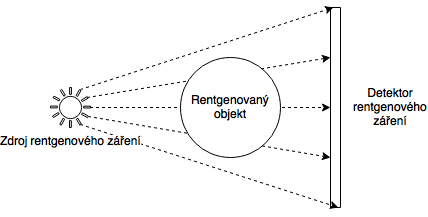
\includegraphics[width=\textwidth]{xray-scene}
\caption{Scéna pro pořizování rentgenových snímků.}
\label{fig:x-ray-scene}
\centering
\end{figure}

\subsection{Rentgenka}
Zdrojem rentgenového záření při pořizování rentgenových snímků je nejčastěji speciální vakuová elektronka, které je často nazývána jako rentgenka, rentgenová lampa či rentgenová trubice. \cite{AstroNuklFyzika-JadRadMetody} Rentgenku si lze představit, jako zařízení, které převádí energii elektronů na elektromagnetické záření s odpovídající energií. Expozice a spektrum záření mlže být řízena nastavením parametrů rentgenky jako jsou napětí (\SI{}{\kilo\volt}), proud (\SI{}{\milli\ampere}) a doba expozice (\SI{}{\second}). \cite[str.~93]{Diagnostic-Radiology-Physics}

\subsubsection{Principy fungování rentgenky}
Princip fungování rentgenky je založen na emitování elektronů žhavenou katodou, které jsou přitahovány k anodě s vysokým kladným napětím. Elektrony jsou silným statickým napětím urychlovány a po dopadu na anodu prudce zabrzdí, přičemž část kinetické energie je přeměněna na brzdné a charakteristické X-záření. \cite{AstroNuklFyzika-JadRadMetody}. Množství emitovaných elektronů může být řízeno změnou proudu žhavení, tedy změnou teploty žhaveného vlákna a tím i množství emitovaných elektronů a změnou potenciálu mezi katodou a anodou měnící energii X-záření. \cite[str.~93]{Diagnostic-Radiology-Physics}

Prudké zabrzdění elektronů je zajištěno materiálem anody. Anoda bývá zhotovena z materiálů s vysokou elektronovou hustotou (nejčastěji wolfram). I přes vysokou elektronovou hustotu materiálu anody je přibližná účinnost procesu přeměny kinetické energie na X-záření pouze 1\%. Zbylá kinetická energie je předávána elektronům a atomům krystalové mřížky a je přeměněna na teplo. \cite[kap. 3.2]{AstroNuklFyzika-JadRadMetody}

\begin{figure}[bh]
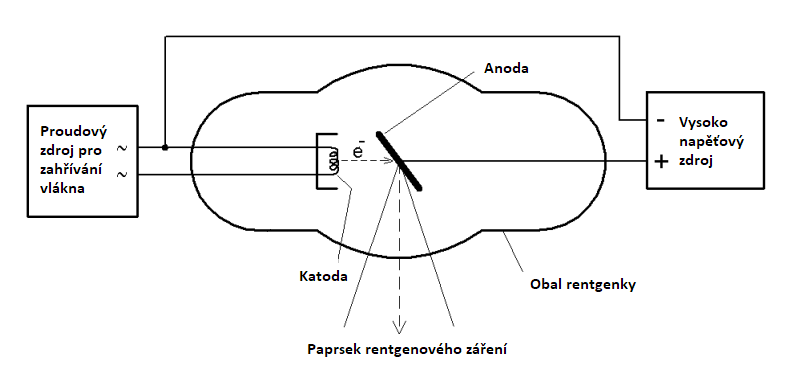
\includegraphics[width=\textwidth]{xray-tube}
\caption{Rentgenka se zdroji proudu a napětí. \cite[str. 93]{Diagnostic-Radiology-Physics}}
\label{fig:x-ray-scene}
\centering
\end{figure}

\subsubsection{Konstrukce rentgenky}
Z důvodu tepelného ohřevu anody po dopadu zrychlených elektronů a vysokého napětí na elektrodách musí být rentgenky oproti běžným elektronkám robustní konstrukce. Chlazení samotné anody je zajištěno její velikostí a také rotací  nebo aktivním chlazením (bude popsáno níže - doplnit referenci!!!). Rentgenky lze rozdělit kategorií podle způsobu využití a konstrukce:
\begin{itemize}
\item Rentgenky pro průmyslové ozařování a radioterapeutické použití - rentgenky s pevnou anodou, kde je chlazení zajištěno průtokem chladícího média. U toho typu rentgenek je častým požadavkem vysoká energie a intenzita záření. Naopak zde není potřebné zaměřování elektronů do téměř bodového ohniska. 
\item Rentgenky pro rentgenovou diagnostiku - rentgenky se soustředěním elektronů do ohniska. U tohoto typu rentgenek se využívá rotující anody proti nadměrnému přehřívání anody v místě ohniska.
\item Speciální rentgenky - rentgenky rozšířené o třetí elektrodu (drátěnou mřížku umístěnou mezi katodou a anodou v těsné blízkosti katody) sloužící k řízení proudu protékajícího anodou. Proud je řízen napětím, které je přivedeno na drátěnou mřížku.
\end{itemize}


